%------------------------------%
%% ✎ Dylan (V1) %%%%%%%%% ✅ %%
%% ✎ Alain (V2) %%%%%%%%% ❌ %%
%% ✎ Dylan (V3) %%%%%%%%% ❌ %%
%------------------------------%

\afterpage{%
\afterpage{%

    % Arrière-plan conclusion generale
    \AddToShipoutPictureBG*{%
\includegraphics[width=\paperwidth,height=\paperheight]{src/Figures/Arriere_plan/Arriere_plan_Conclusion.jpg}
    }

% Rectangle
\AddToShipoutPictureBG*{
  \begin{tikzpicture}[remember picture,overlay]
    \node[fill=white, opacity=0.75, text width=\paperwidth, minimum height=5cm, anchor=north] 
    at ([yshift=-9cm]current page.north) {};
  \end{tikzpicture}
}

% Source
\AddToShipoutPictureFG*{
  \AtPageLowerRight{
    \raisebox{1cm}{
      \hspace{16cm}
      
\begin{tikzpicture}
        \node[fill=white, rounded corners=5pt, inner sep=5pt, align=center] {
          \tiny{Photographie~: \textcolor{blue}{Dylan Moinse (2020)}}
        };
      \end{tikzpicture}
    }
  }
}
}}

\renewcommand{\thefigure}{C.\arabic{figure}} % Numérotation spécifique pour la conclusion
\renewcommand{\thetable}{C.\arabic{table}}
\setcounter{figure}{0}

    \needspace{1\baselineskip} % Réserve de l'espace
\part*{Conclusion générale}
    %\addcontentsline{toc}{part}{Conclusion générale}
    \label{body:conclusion-generale}
    \markboth{Conclusion générale}{}
    \markright{Conclusion générale}{}
    \begin{refsegment}

    % Problématique
\lettrine[lines=3, findent=8pt, nindent=0pt]{\lettrinefont N}{ous} nous sommes attachés à interroger la contribution de la mobilité individuelle légère au renforcement du \acrshort{TOD}. Sur la base d'une investigation sur la trame régionale des quartiers de gare, dans les Hauts-de-France, nous avons été en mesure d'évaluer la pertinence et le potentiel de la mobilité individuelle légère à répondre aux enjeux des \Guillemets{premiers et derniers kilomètres} et à préparer le terrain pour un \acrfull{M-TOD}, ou un urbanisme orienté vers les réseaux de transport en commun et intégrant la mobilité individuelle légère. En revenant sur notre \hyperref[introduction-generale:problematique-objectifs-hypotheses]{problématique de recherche} (page~\pageref{introduction-generale:problematique-objectifs-hypotheses}), nous avons tenté à déterminer l'apport de la mobilité individuelle légère dans l'amélioration de l'\gls{accessibilité intermodale}, les transformations spatiales induites par ces proximités redéfinies, ainsi que les stratégies d'aménagement et de mobilité en vue de promouvoir un modèle \acrshort{M-TOD}.

    % Principaux enseignements
En regroupant les principales leçons tirées, nous avons démontré que la mobilité individuelle légère constitue un mode de transfert efficace en connexion avec les pôles d'échange, permettant non seulement de consolider l'\gls{accessibilité}, au niveau local, dans les espaces dans lesquels les services de \gls{transport en commun} peinent à assurer une couverture fine, mais aussi de renforcer l'accessibilité, au niveau régional. En étendant l’aire d’influence des quartiers de gare, la mobilité individuelle légère rend les déplacements intermodaux plus compétitifs face à l’usage de l'automobile, en particulier dans les territoires où les conditions de circulation et de stationnement sont contraignantes. Nos résultats mettent également en évidence le fait que cette complémentarité modale ne peut être pleinement opérante sans une reconfiguration des structures spatiales. Si certaines interventions sont requises à proximité directe des nœuds de transport en commun, elles sont d’autant plus incontournables à l’échelle des quartiers de gare étendus, où l’organisation territoriale reste souvent inadaptée à la pratique cyclable. L’un des apports majeurs de cette thèse réside ainsi dans la démonstration que l’intégration de la mobilité individuelle légère dans le concept d'aménagement du \acrshort{TOD} ne constitue pas une amélioration marginale, mais bien une transformation structurelle du modèle d’urbanisme ferroviaire. Cette évolution appelle à repenser la planification des quartiers de gare, à différentes échelles spatiales, en mettant à profit les atouts de la mobilité individuelle légère afin de développer un système urbain adapté aux enjeux de la mobilité contemporaine.%%Rédigé%%

    % Transition hypothèses
En guise de bilan critique, cette conclusion revient sur les objectifs et les hypothèses de recherche définis dans l’\hyperref[body:introduction-generale]{introduction générale} (page~\pageref{body:introduction-generale}) et explorés tout au long de ce travail doctoral. Il s’agit, en outre, de confronter les résultats obtenus aux résultats attendus, en présentant les principaux enseignements tirés de notre recherche. Notre démarche consiste ainsi à \Guillemets{corroborer} ou à invalider nos hypothèses à la lumière des résultats empiriques\footnote{
    Comme le rapportent \textcolor{blue}{\textcite[44]{tomini_methodes_2020}}\index{Tomini, Luca|pagebf}\index{Wintgens, Sophie|pagebf}, il convient de rappeler \Guillemets{l'impossible validation des hypothèses}. En effet, une hypothèse scientifique ne peut être que réfutée, mais jamais entièrement validée. Cette position épistémologique en sciences sociales, ou \Guillemets{la fin de la certitude scientifique} \textcolor{blue}{\autocite[303]{baraquin_popper_2020}}\index{Baraquin, Noëlla|pagebf}\index{Laffitte, Jacqueline|pagebf}, est précisément celle dictée par l'enseignant en philosophie des sciences \textcolor{blue}{Karl~R.} \textcolor{blue}{\textcite[273]{popper_logique_1973}}\index{Popper, Karl~R.|pagebf}, selon laquelle une hypothèse ne peut être considérée comme définitivement vraie. Il est seulement possible d'affirmer qu'elle n'a pas encore été rejetée, et de la tenir donc pour vraie jusqu'à preuve du contraire. Ainsi, une hypothèse ne possède pas un degré de corroboration positif absolu, dès lors qu'elle est falsifiée~: c'est le \Guillemets{principe de réfutabilité}.
} \textcolor{blue}{\autocite[44]{tomini_methodes_2020}}\index{Tomini, Luca|pagebf}\index{Wintgens, Sophie|pagebf}, dans le respect du \Guillemets{principe de réfutabilité} \textcolor{blue}{\autocite[273]{popper_logique_1973}}\index{Popper, Karl~R.|pagebf}. Dans cette perspective, l'exercice qui suit propose une synthèse des principaux apports de la recherche, en lien avec nos hypothèses, qui ont alors reposé sur une double approche inductive et hypothético-déductive. Cette démarche ayant permis d'opérer des \Guillemets{va-et-vient} entre les concepts et les réalités sociales, de façon à garantir la richesse de notre démarche géographique \textcolor{blue}{\autocite[24]{ageron_intermodalite-voyageurs_2013}}\index{Ageron, Pierre|pagebf}\index{Varlet, Jean|pagebf}.%%Rédigé%%

% --- %
    \newpage
    \needspace{2\baselineskip} % Réserve de l'espace
\section*{Synthèse des principaux apports de la recherche doctorale
    \label{conclusion-generale:principaux-apports}
    }
    \addcontentsline{toc}{section}{Synthèse des principaux apports de la recherche doctorale}
    %\markboth{Synthèse des principaux apports de la recherche doctorale}{}
    \markright{Synthèse des principaux apports de la recherche doctorale}{}

    \needspace{1\baselineskip} % Réserve de l'espace
\subsubsection*{Déclinaisons du concept d'aménagement
    \label{conclusion-generale:principaux-apports-chapitre1}
    }

    % Objectif 1 - Hypothèse 1 - part 1
\hyperref[objectif-1]{Le premier objectif de recherche} (\(O_1\), page~\pageref{objectif-1}) consistait à justifier la pertinence d'un modèle réactualisé prenant en compte la composante intermodale impliquant l'usage de la mobilité individuelle, soit un \acrshort{M-TOD}. En cela, \hyperref[chap1:titre]{le premier chapitre} (page~\pageref{chap1:titre}) a permis de soulever les enjeux contemporains du \acrshort{TOD}, en posant les bases conceptuelles et historiques de ce modèle d'aménagement (voir le \hyperref[table-conclusion:confrontation-hypotheses]{tableau~\ref{table-conclusion:confrontation-hypotheses}} à la page~\pageref{table-conclusion:confrontation-hypotheses} et le \hyperref[fig-conclusion:synthese-enseignements]{schéma~\ref{fig-conclusion:synthese-enseignements}} à la page~\pageref{fig-conclusion:synthese-enseignements}). Au cours de cette démonstration mettant en récit ses évolutions et ses adaptations, nous avons mis en relief l'un des défis majeurs auxquels il est confronté aujourd'hui~: la problématique majeure des \Guillemets{premiers et derniers kilomètres}. Nous avons pu démontrer combien la mobilité individuelle légère représente une ressource stratégique, à la fois plus résiliente et moins contraignante que nombre d'innovations actuellement mises en avant, notamment celles centrées sur l'automobile. Cette approche systémique de la mobilité promeut ainsi une intelligence des flux et des réseaux, et constitue le cœur de notre cadre théorique.%%Rédigé%%

    % Objectif 1 - Hypothèse 1 - part 2
Il s'agit plus précisément de mobiliser la récente conceptualisation d'un \acrfull{B-TOD}. L'enjeu a été de resituer la diversification modale récente du \gls{vélo} et de la \gls{micro-mobilité}, qui vient enrichir cette déclinaison originellement centrée sur le vélo conventionnel. Nous y intégrons une multiplicité de solutions intermodales émergentes, allant de la portabilité des véhicules et de l'essor de l'électromobilité légère, à la mise en service de ces véhicules dans les espaces publics. Cette diversification permet ainsi d’étendre le champ des solutions intermodales, en répondant de manière plus adaptée et flexible aux besoins de mobilité exprimés dans les territoires. En conséquence, nous avons démontré que, pris séparément, les deux objets d’étude que nous cherchons à croiser~–~le \acrshort{TOD} et la mobilité individuelle légère~–~suscitent un intérêt croissant, tant dans la recherche que dans les opérations d'aménagement (\hyperref[sous-hypothese-1.1]{\(S.H_{1.1}\)}, page~\pageref{sous-hypothese-1.1}). Pourtant, nous observons que ces deux sujets font rarement l'objet d'une analyse conjointe, alors même que la maximisation de leur efficacité tient à la force de leur interaction. C’est précisément ce manque de convergence qui justifie l’intérêt de cette recherche et la nécessité de combler cette lacune conceptuelle et opérationnelle (\hyperref[sous-hypothese-1.2]{\(S.H_{1.2}\)}, page~\pageref{sous-hypothese-1.2}).%%Rédigé%%

    % Tableau confrontation hypothèses de recherche
% Tableau confrontation des hypothèses de recherche

    \begin{table}[h!]
    \centering
    \renewcommand{\arraystretch}{1.5}
    \resizebox{\columnwidth}{!}{
    \begin{tabular}{p{0.01\columnwidth}p{0.495\columnwidth}p{0.495\columnwidth}}
        %\hline
    \rule{0pt}{15pt} \small{\textbf{\textcolor{blue}{}}} & \small{\textbf{\textcolor{blue}{Résultats attendus}}} & \small{\textbf{\textcolor{blue}{Résultats observés}}}\\
        \hline
\cellcolor{green!20} & \textbf{Hypothèse 1} \small{(\hyperref[hypothese-1]{\(H_{1}\)}, page~\pageref{hypothese-1})} & \cellcolor{green!20}\textbf{\small{Corroborée}}\\
\cellcolor{green!20} & \small{\textsl{L’émergence de nouvelles thématiques de recherche sur le Transit-Oriented Development et la mobilité individuelle légère appelle une analyse conjointe.}} & \small{Si ces deux objets d’étude suscitent un intérêt croissant, ils sont encore trop souvent abordés séparément, alors que leur synergie offre des éclairages pertinents.}\\
    \hdashline
\cellcolor{orange!20} & \textbf{Hypothèse 2} \small{(\hyperref[hypothese-2]{\(H_{2}\)}, page~\pageref{hypothese-2})} & \cellcolor{orange!20}\textbf{\small{Partiellement invalidée}}\\
\cellcolor{orange!20} & \small{\textsl{Les recherches sur cette synergie intermodale restent conditionnées par l’association vélo et train et sont rarement mises en relation avec le concept d'aménagement.}} & \small{Le \textsl{Transit-Oriented Development} est souvent convoqué dans les études, bien qu'il soit inadéquatement exploité, et l’intégration des nouvelles solutions de mobilité devient un sujet d’étude croissant, hormis dans les contextes européens.}\\
    \hdashline
\cellcolor{orange!20} & \textbf{Hypothèse 3} \small{(\hyperref[hypothese-3]{\(H_{3}\)}, page~\pageref{hypothese-3})} & \cellcolor{orange!20}\textbf{\small{Partiellement invalidée}}\\
\cellcolor{orange!20} & \small{\textsl{La complexité des interactions entre réseau et territoire appelle une méthodologie systémique, capable de produire des résultats allant au-delà d'une simple juxtaposition.}} & \small{La complémentarité des approches a non seulement permis de générer de nouveaux questionnements, mais elle aussi su structurer une démarche multidimensionnelle et multiscalaire, non sans échapper à des risques de superposition et de contrainte temporelle.}\\
    \hdashline
\cellcolor{green!20} & \textbf{Hypothèse 4} \small{(\hyperref[hypothese-4]{\(H_{4}\)}, page~\pageref{hypothese-4})} & \cellcolor{green!20}\textbf{\small{Corroborée}}\\
\cellcolor{green!20} & \small{\textsl{Les pratiques intermodales, impliquant l'usage de la mobilité individuelle légère, s’intensifient sous l’effet de l'essor de la micro-mobilité, en dépit d'une appropriation inégalitaire par certains groupes sociaux.}} & \small{La mobilité individuelle légère, en tant que mode de transfert, connaît une \Guillemets{émergence} principalement portée par l'adoption de la trottinette électrique à usage personnel. Toutefois, son usage intermodal est plus inégalitaire qu'en monomodalité, bien que des interventions par l'urbanisme jouent un rôle modérateur sur les inégalités de genre.} \\
    \hdashline
\cellcolor{green!20} & \textbf{Hypothèse 5} \small{(\hyperref[hypothese-5]{\(H_{5}\)}, page~\pageref{hypothese-5})} & \cellcolor{green!20}\textbf{\small{Corroborée}}\\
\cellcolor{green!20} & \small{\textsl{Grâce à l’intégration de la mobilité individuelle légère, l’accessibilité multiscalaire par les transports en commun devient nettement plus performante, résiliente et compétitive.}} & \small{Les quartiers de gare accessibles à l'aide de la mobilité individuelle légère bénéficient d’une extension locale de leur périmètre et une augmentation des opportunités d’accès aux ressources régionales. Les choix d’itinéraire sont influencés par des stratégies de détour et de pause, qui, grâce à la portée et à la flexibilité offertes par ces véhicules, optimisent le déplacement intermodal.}\\
    \hdashline
\cellcolor{green!20} & \textbf{Hypothèse 6} \small{(\hyperref[hypothese-6]{\(H_{6}\)}, page~\pageref{hypothese-6})} & \cellcolor{green!20}\textbf{\small{Corroborée}}\\
\cellcolor{green!20} & \small{\textsl{Associer la mobilité individuelle légère aux stratégies d'aménagement représente une opportunité pour intégrer et étendre les quartiers de gare, mais aussi pour stimuler la fréquentation des transports en commun.}} & \small{Parmi les principaux leviers d’action en faveur d’un urbanisme orienté vers le rail, figure l’amélioration de la connectivité locale, avec un accent particulier sur les investissements dans le \Guillemets{système vélo} afin de dynamiser la fréquentation des gares, en appui aux orientations du \acrshort{TOD}.}\\
        \hline
        \end{tabular}}
    \caption{Test des hypothèses de recherche en fonction des conclusions de la recherche.}
    \label{table-conclusion:confrontation-hypotheses}
        \vspace{5pt}
        \begin{flushright}\scriptsize{
        Auteur~: \textcolor{blue}{Dylan Moinse (2025)}
        }\end{flushright}
        \end{table}

    \needspace{1\baselineskip} % Réserve de l'espace
\subsubsection*{Synthèse des connaissances actuelles
    \label{conclusion-generale:principaux-apports-chapitre2}
    }

    % Objectif 2 - Hypothèse 2 - part 1
\hyperref[objectif-2]{Le deuxième objectif de recherche} (\(O_2\), page~\pageref{objectif-2}) vise à synthétiser de manière critique les connaissances existantes et les expériences internationales sur ce sujet de recherche. À cette fin, \hyperref[chap2:titre]{le deuxième chapitre} (page~\pageref{chap2:titre}) a recensé l'état actuel de la littérature scientifique et technique sur le \acrshort{B-TOD} et le \acrshort{M-TOD}. Toutefois, si ces concepts émergent implicitement dans les travaux analysés, presque aucune étude ne les revendique formellement, à la différence du \acrshort{TOD}, largement cité et utilisé comme cadre d'analyse (voir le \hyperref[table-conclusion:confrontation-hypotheses]{tableau~\ref{table-conclusion:confrontation-hypotheses}} à la page~\pageref{table-conclusion:confrontation-hypotheses} et le \hyperref[fig-conclusion:synthese-enseignements]{schéma~\ref{fig-conclusion:synthese-enseignements}} à la page~\pageref{fig-conclusion:synthese-enseignements}). L’analyse bibliométrique a révélé un intérêt en très forte croissance pour ces thématiques, avec un doublement du corpus au cours des cinq dernières années. Nous avons notamment identifié quatre regroupements principaux de co-auteur·rice·s qui concentrent une part importante des références bibliographiques répertoriées, au sein de l'Europe occidentale, de l'Asie de l'Est et des États-Unis. La \acrfull{RSL} a également permis d’identifier une évolution temporelle et géographique des combinaisons modales. Au départ, les recherches étaient dominées par le couple vélo et train, notamment dans le Vieux Continent, au cours des deux décennies ayant suivi la formalisation du \acrshort{TOD}. Ensuite, un glissement s’est opéré vers l'étude de la complémentarité entre le \acrfull{VLS} et le train. Plus récemment, ces dynamiques se sont accélérées avec l’essor du \acrfull{VFF} et de la \acrfull{TEFF}, associées au métro. Cette transition est particulièrement visible dans les deux autres régions du monde mentionnées (\hyperref[sous-hypothese-2.1]{\(S.H_{2.1}\)}, page~\pageref{sous-hypothese-2.1}).%%Rédigé%%

    % Objectif 2 - Hypothèse 2 - part 2
Sur le plan méthodologique, la collecte des données s’est profondément transformée pour s’adapter aux évolutions des systèmes connectés. L’exploitation de la \textsl{Big Data}, combinée à des approches basées sur la statistique et la modélisation avancées, tend progressivement à éclipser les méthodes d’enquête de terrain traditionnelles. Concernant les résultats les plus fréquemment rapportés, la \acrshort{RSL} a mis en évidence l’influence positive de la densité de population et des emplois ainsi que la diversité de l'usage des sols, et le traitement des espaces publics. Ces éléments confirment la compatibilité entre l'usage intermodal de la mobilité individuelle légère et les principes premiers du \acrshort{TOD}. Certaines insuffisances ont été identifiées à l’issue de cette revue de littérature. D'une part, une quasi-absence des travaux sur la micro-mobilité et sur les différentes déclinaisons du vélo à usage personnel, en dehors des analyses sur le vélo conventionnel. D'autre part, la rareté des études adoptant une échelle régionale, pourtant structurante dans la pensée du \acrshort{TOD}. Enfin, bien que le \acrshort{TOD} soit fréquemment mentionné, l'articulation entre réseau et territoire est peu étudiée. L’approche territoriale est largement marginalisée, au profit d’une lecture centrée exclusivement sur les infrastructures et les services de transport (\hyperref[sous-hypothese-2.2]{\(S.H_{2.2}\)}, page~\pageref{sous-hypothese-2.2}).%%Rédigé%%

    \needspace{1\baselineskip} % Réserve de l'espace
\subsubsection*{Cheminement méthodologique
    \label{conclusion-generale:principaux-apports-chapitre3}
    }

    % Objectif 3 - Hypothèse 3 - part 1
\hyperref[objectif-3]{Le troisième objectif de recherche} (\(O_3\), page~\pageref{objectif-3}) vise à s'emparer d'une méthodologie mixte permettant d'appréhender ce sujet complexe qui embrasse une pluralité de thématiques et d'échelles territoriales. \hyperref[chap3:titre]{Le troisième chapitre} (page~\pageref{chap3:titre}) a ainsi été l’occasion de définir une \Guillemets{enquête sur-mesure}, combinant des approches quantitatives et qualitatives adaptées à un sujet de recherche à la fois multidimensionnel et multiscalaire (voir le \hyperref[table-conclusion:confrontation-hypotheses]{tableau~\ref{table-conclusion:confrontation-hypotheses}} à la page~\pageref{table-conclusion:confrontation-hypotheses} et le \hyperref[fig-conclusion:synthese-enseignements]{schéma~\ref{fig-conclusion:synthese-enseignements}} à la page~\pageref{fig-conclusion:synthese-enseignements}). La structuration méthodologique s’appuie sur l’articulation de plusieurs outils complémentaires~: l’enquête par observation directe et par questionnaire, des entretiens \textsl{in situ}, ainsi que le recours à des outils d'analyse géostatistique et à la modélisation spatiale. Ces recherches mixtes ont permis d’adopter une démarche progressive et structurée, en s’appuyant sur les différentes facettes de la notion d’\Guillemets{accessibilité}. L’objectif était ainsi de produire un matériau empirique original, nous permettant d'aborder la complexité de la mobilité quotidienne et des interrelations entre réseau et territoire. En premier lieu, l’enquête par observation quantitative a permis d'étayer le caractère \Guillemets{émergent} des pratiques intermodales impliquant la mobilité individuelle légère en gare. Elle a également permis de caractériser le profil socio-démographique des utilisateur·rice·s, tout en croisant ces résultats avec des bases de données existantes, afin d’établir une mise en perspective avec les agencements de l’environnement urbain. L’enquête par questionnaire a complété cette approche en apportant des informations détaillées sur les comportements de mobilité et les motivations des cyclo-voyageur·se·s. Elle a aussi contribué à la cartographie des itinéraires empruntés, offrant une lecture plus fine des interrelations entre pratiques intermodales, espaces et lieux. Cette démarche nous a ainsi permis d'entrer plus en détail sur les dimensions mobilitaires et territoriales de ces pratiques de mobilité, en lien avec notre problématique de recherche. De plus, la conduite de parcours commentés a offert une perspective plus compréhensive sur la \gls{perception} des usager·ère·s vis-à-vis de leurs comportements, des conditions d’accessibilité et des obstacles rencontrés. L'intention de croiser les méthodes a alors permis d’articuler l'emploi de la statistique avec l’analyse de discours et d'images.%%Rédigé%%

    % Objectif 3 - Hypothèse 3 - part 2
Enfin, grâce au travail de modélisation spatiale, nous avons pu développer une analyse plus systémique des phénomènes étudiés, en intégrant les facteurs déterminants identifiés dans la \acrfull{RSL} ainsi que les enseignements exploratoires tirés de l’investigation de terrain. Ce modèle revisité a permis d’examiner la coordination des différentes composantes du \acrshort{TOD}, afin de poser les bases du \acrshort{M-TOD}. Dès lors, comme le souligne \textcolor{blue}{Hélène} \textcolor{blue}{\textcite{nessi_traduire_2022}}\index{Nessi, Hélène|pagebf}, l’intérêt de cette combinaison méthodologique réside non pas dans une subordination d’une approche à l’autre, mais bien dans leur dialogue, permettant d’aboutir à une contextualisation plus riche des données et à l’émergence de nouvelles hypothèses (\hyperref[sous-hypothese-3.1]{\(S.H_{3.1}\)}, page~\pageref{sous-hypothese-3.1}). L’application de cette méthodologie a ainsi permis de définir et de délimiter le terrain géographique de l’étude, basé à la fois sur le système ferroviaire de la région Hauts-de-France et sur ses \Guillemets{quartiers de gare}, vus sous l’angle de la marche combinée et de la mobilité individuelle légère. La stratégie multiscalaire suivie permet de dépasser une lecture strictement locale ou macro-régionale, en capturant la complexité des systèmes de mobilité et des dynamiques territoriales. Cette modélisation spatiale et ce jeu d’échelles ayant, à leur tour, été rendus possibles grâce à la collecte et au traitement des données géographiques issues de l’administration du questionnaire auprès des cyclo-voyageur·se·s (\hyperref[sous-hypothese-3.2]{\(S.H_{3.2}\)}, page~\pageref{sous-hypothese-3.2}).%%Rédigé%%

    \needspace{1\baselineskip} % Réserve de l'espace
\subsubsection*{Caractérisation des individus mobiles
    \label{conclusion-generale:principaux-apports-chapitre4}
    }

    % Objectif 4 - Hypothèse 4 - part 1
\hyperref[objectif-4]{Le quatrième objectif de recherche} (\(O_4\), page~\pageref{objectif-4}) vise à quantifier et à caractériser les pratiques intermodales, en s'intéressant au profil des usager·ère·s combinant l'usage de la mobilité individuelle et des transports en commun, ainsi qu'aux facteurs socio-démographiques et aux ressources dont iels disposent (voir le \hyperref[table-conclusion:confrontation-hypotheses]{tableau~\ref{table-conclusion:confrontation-hypotheses}} à la page~\pageref{table-conclusion:confrontation-hypotheses} et le \hyperref[fig-conclusion:synthese-enseignements]{schéma~\ref{fig-conclusion:synthese-enseignements}} à la page~\pageref{fig-conclusion:synthese-enseignements}). \hyperref[chap4:titre]{Le quatrième chapitre} (page~\pageref{chap4:titre}) a permis d'estimer la part modale de la mobilité individuelle légère en transfert avec le train, représentant environ 8~\% des flux de voyageur·se·s observés en gare. Cette proportion s'explique notamment par l'essor de la \acrfull{TEP}, qui atteint une part de 3~\%, tandis que le vélo classique détient quant à lui une proportion similaire. L'approche comparative des parts modales renseignées révèle un intérêt croissant pour la mobilité individuelle légère dans les territoires périurbains, à condition que les gares disposent d'un niveau de service minimal. L'hypothèse selon laquelle ces pratiques intermodales sont bien présentes et en pleine expansion a été confirmée~: plus d'un tiers des cyclo-voyageur·se·s, et même la moitié d'entre elleux pour les systèmes de partage, la \acrshort{TEP}, le \acrfull{VAE} et le vélo pliant, déclarent avoir adopté ces combinaisons modales depuis moins d'un an (\hyperref[sous-hypothese-4.1]{\(S.H_{4.1}\)}, page~\pageref{sous-hypothese-4.1}). Plus de la moitié des usager·ère·s intermodaux·les utilisent ces combinaisons modales quasi quotidiennement, et trois quarts des cyclo-voyageur·se·s sont des navetteur·se·s. Nous avons également pu mettre en évidence un renoncement au bus de rabattement et à l'automobile au profit de la mobilité individuelle légère combinée. Par ailleurs, il apparaît qu'une part significative des usager·ère·s renoncerait complètement à l’usage du train en cas d’indisponibilité de ces véhicules légers. Enfin, les véhicules pliants présentent un avantage comparatif en ce qu’ils sont plus fréquemment utilisés à la fois en pré-acheminement et en post-acheminement.%%Rédigé%%

    % Objectif 4 - Hypothèse 4 - part 2
Partant de ces informations sur les comportements de mobilité, nous avons pu saisir les traits caractéristiques de ce groupe social en révélant une surreprésentation des hommes adultes, occupant des emplois de cadre supérieur et disposant d’un niveau de qualification et de revenus relativement plus élevés. Les femmes ne représentent qu'un quart des usager·ère·s, notamment en ce qui concerne le vélo et la \acrshort{TEP}, tandis que la moitié des répondant·e·s a moins de 33 ans. De surcroît, à mesure que l’âge augmente, les inégalités de \gls{genre} se creusent, en défaveur des femmes~: il y a là un double effet de genre et d'âge. L’étude a ainsi permis de conforter le constat de l’existence d’inégalités de genre dans l’usage du vélo et de la micro-mobilité, d'autant plus prononcées en situation d'\gls{intermodalité}, en France. En croisant ces résultats avec des bases de données, une association positive, statistiquement significative, a été néanmoins mise en évidence~: entre la part modale du vélo, le niveau de cyclabilité objective et perçue, et la proportion de femmes cyclistes. Ces résultats démontrent que l’atteinte d’un usage paritaire du vélo dépasse les seules considérations liées à la masse critique de cyclistes ou à la présence d’infrastructures cyclables. En réalité, le principal déterminant réside dans la cyclabilité perçue. En d'autres termes, il s'agit principalement d'améliorer le \Guillemets{système vélo} (\hyperref[sous-hypothese-4.2]{\(S.H_{4.2}\)}, page~\pageref{sous-hypothese-4.2}).%%Rédigé%%

    \needspace{1\baselineskip} % Réserve de l'espace
\subsubsection*{Mesure des gains d'accessibilité intermodale
    \label{conclusion-generale:principaux-apports-chapitre5}
    }

    % Objectif 5 - Hypothèse 5 - part 1
\hyperref[objectif-5]{Le cinquième objectif de recherche} (\(O_5\), page~\pageref{objectif-5}) s’attache à mesurer et à expliquer l’extension spatiale des quartiers de gare induite par la mobilité individuelle légère, dans le but d’évaluer les gains d’accessibilité intermodale qu’elle permet. En s’inscrivant dans une approche par l'\Guillemets{accessibilité effective}, qui vise à diagnostiquer les conditions d’accessibilité réelles, \hyperref[chap5:titre]{le cinquième chapitre} (page~\pageref{chap5:titre}) se focalise sur les distances spatio-temporelles parcourues par les usager·ère·s, afin de déterminer dans quelle mesure les quartiers de gare s’étendent à l’échelle locale (voir le \hyperref[table-conclusion:confrontation-hypotheses]{tableau~\ref{table-conclusion:confrontation-hypotheses}} à la page~\pageref{table-conclusion:confrontation-hypotheses} et le \hyperref[fig-conclusion:synthese-enseignements]{schéma~\ref{fig-conclusion:synthese-enseignements}} à la page~\pageref{fig-conclusion:synthese-enseignements}). Il examine également les facteurs influençant l’optimisation des cheminements cyclables ainsi que les gains d’accessibilité qui en découlent. L’analyse a permis d’établir que, pour les flux pendulaires, la distance acceptable en \gls{rabattement} comme en \gls{diffusion} s’élève à un kilomètre pour la marche combinée, et à quatre kilomètres pour la mobilité individuelle légère, ce qui correspond à un budget temporel moyen de douze minutes. Cette extension spatiale se traduit par un triplement de la superficie des quartiers de gare accessibles à pied, tandis qu’avec la mobilité individuelle légère, ces derniers s’étendent jusqu’à 23 fois plus que les aires d’influence traditionnellement admises. À l’échelle des déplacements intermodaux, la distance médiane d’un trajet combinant mobilité individuelle légère et train atteint 35 kilomètres, pour une durée moyenne de 53 minutes. Le rayon d’action pertinent pour ce type de \gls{déplacement} varie selon les étapes du trajet, oscillant entre un et quatre kilomètres en pré-acheminement et entre un et trois kilomètres en post-acheminement. Ces distances sont toutefois modulées par l’attractivité des gares, celles bénéficiant des meilleurs services affichant une portée effective de cinq kilomètres, contre quatre kilomètres pour les gares proposant un service de niveau intermédiaire ou plus faible.%%Rédigé%%

    % Objectif 5 - Hypothèse 5 - part 2
L’étude met en évidence une amélioration significative du taux d’accessibilité grâce à l’usage de la mobilité individuelle légère. 60~\% des résident·e·s ont potentiellement accès aux gares par ce biais, et 70~\% du marché de l’emploi devient accessible, soit une multiplication par trois du nombre d’individus et par deux du nombre d’emplois atteignables par rapport à la seule marche combinée. Ce potentiel s’observe également dans l’accès aux équipements et services, puisque le potentiel d’accès aux \acrfull{POIs} double, avec une couverture des deux tiers des équipements disponibles dans la région. Cette amélioration est particulièrement marquée pour les infrastructures de catégorie \Guillemets{supérieure}, dont 80~\% deviennent accessibles, contre 70~\% pour les équipements \Guillemets{intermédiaires} et 60~\% pour ceux de \Guillemets{proximité} (\hyperref[sous-hypothese-5.1]{\(S.H_{5.1}\)}, page~\pageref{sous-hypothese-5.1}). Les choix d’\gls{itinéraire} des usager·ère·s montre que les déplacements ne suivent pas systématiquement les tracés les plus directs localement, mais intègrent des détours, en rabattement et, ou bien, en diffusion, qui peuvent être jusqu’à trois fois plus longs que le parcours supposé. Cette stratégie permet néanmoins de réduire de moitié le temps passé dans les transports en commun et de diminuer de 80~\% le temps d’attente. L’optimisation spatio-temporelle des déplacements par le biais du \gls{détour} se traduit ainsi par une économie de distance-temps et de distance spatiale. Ces détours s’accompagnent fréquemment d’une meilleure rationalisation du temps de parcours, en intégrant des pauses stratégiques~: ces interruptions sont souvent mises à profit pour des achats du quotidien, suggérant que ces déplacements s’inscrivent dans des chaînes de mobilité plus complexes, où la mobilité individuelle légère joue un rôle central dans l’articulation entre transport public et activités quotidiennes (\hyperref[sous-hypothese-5.2]{\(S.H_{5.2}\)}, page~\pageref{sous-hypothese-5.2}).%%Rédigé%%

    \needspace{1\baselineskip} % Réserve de l'espace
\subsubsection*{Modélisation spatiale et action par l'urbanisme
    \label{conclusion-generale:principaux-apports-chapitre6}
    }

    % Objectif 6 - Hypothèse 6 - part 1
\hyperref[objectif-6]{Le sixième objectif de recherche} (\(O_6\), page~\pageref{objectif-6}) s'oriente vers la détection des paramètres à privilégier pour développer efficacement un \acrfull{M-TOD}. À la différence des chapitres antérieurs, fondés sur une approche par l'\Guillemets{accessibilité effective}, ce dernier volet de la recherche doctorale se penche sur l'\Guillemets{accessibilité normative}, cherchant à formuler des préconisations pour améliorer l’accessibilité, tout en garantissant leur faisabilité \textcolor{blue}{\autocite[19]{levine_mobility_2019}}\index{Levine, Jonathan|pagebf}\index{Grengs, Joe|pagebf}\index{Merlin, Louis~A.|pagebf}. Cette approche prescriptive s’appuie néanmoins sur les enseignements tirés de l’\Guillemets{accessibilité effective}, en intégrant les conditions réelles d’accessibilité identifiées. \hyperref[chap6:titre]{Le sixième chapitre} (page~\pageref{chap6:titre}) repose sur une modélisation spatiale destinée à évaluer l’impact des différents critères contribuant à la définition d’un \acrshort{TOD}, intégrant une portée étendue de la marche combinée, et d'un \acrshort{M-TOD} (voir le \hyperref[table-conclusion:confrontation-hypotheses]{tableau~\ref{table-conclusion:confrontation-hypotheses}} à la page~\pageref{table-conclusion:confrontation-hypotheses} et le \hyperref[fig-conclusion:synthese-enseignements]{schéma~\ref{fig-conclusion:synthese-enseignements}} à la page~\pageref{fig-conclusion:synthese-enseignements}). Une grille d'analyse structurée à partir de quatre dimensions clés dessine les contours du modèle \acrfull{NPART}~: la forme du réseau et la qualité de ses services (\(N\))~; le degré de développement urbain (\(P\))~; les connexions locales et le traitement des espaces publics (\(A\))~; et la fréquentation temporelle des gares, segmentée par heure et par période (\(RT\)). L’analyse de ces critères, aussi bien du point de vue de la formalisation conceptuelle que de l’opérationnalisation des principes du \acrshort{M-TOD}, a permis d’élaborer des recommandations à destination des acteurs de la fabrique urbaine. Il apparaît que les critères les plus déterminants pour l’attractivité des gares, et donc pour la stimulation de la demande prédite, sont en grande partie liés à la connectivité locale dans les quartiers de gare. Plus précisément, la qualité de la desserte en métro et en tramway joue un rôle central, mais cette dynamique est largement renforcée par la présence d’infrastructures dédiées au développement du vélo, telles que les services de \acrfull{VLS}, les espaces de stationnement ainsi que l'aménagement d'un réseau cyclable. Ces éléments représentent de ce fait des facteurs structurants de quartiers \acrshort{TOD}\textcolor{blue}{s} et \acrshort{M-TOD}\textcolor{blue}{s}, en particulier aux heures de pointe, tant à l’échelle piétonne qu’à l’échelle cyclable.%%Rédigé%%

    % Objectif 6 - Hypothèse 6 - part 2
De plus, ce panorama des principaux indicateurs définissant ces stratégies urbaines met aussi en lumière un décalage avec les orientations stratégiques privilégiées par les aménageur·se·s en France. En effet, ces dernier·ère·s tendent à concentrer leurs efforts sur l’accès aux centralités urbaines, sur la spécialisation commerciale des territoires, sur le développement des cheminements piétons, ainsi que sur la limitation de la vitesse motorisée et sur la réduction de la possession automobile, des objectifs qui, bien que pertinents, ne répondent que partiellement aux enjeux d’accessibilité (\hyperref[sous-hypothese-6.1]{\(S.H_{6.1}\)}, page~\pageref{sous-hypothese-6.1}). L’aboutissement du modèle \acrshort{NPART} a conduit à une classification des gares et de leurs aires d’influence, permettant d’identifier trois classes distinctes en fonction de leur potentiel d’intégration au modèle \acrshort{M-TOD}. Cette analyse a révélé que la majorité des gares étudiées présentent des caractéristiques propices au développement d’un \acrshort{M-TOD} incorporant le \acrshort{TOD}, mais souffrent d’un manque criant de connexions piétonnes et cyclables, les plaçant pour la plupart dans une dynamique plus proche du \acrfull{TAD}. Ainsi, en l’absence d’un véritable traitement des espaces publics, ces gares peinent à tirer parti de la qualité de leur service ferroviaire ou de la polarisation des activités humaines. L’un des enseignements majeurs de ce modèle avancé est alors que la promotion d’un \Guillemets{système vélo} renforce considérablement la capacité des quartiers de gare à accroître la fréquentation ferroviaire. Par ailleurs, nous avons pu observer que l'extension des quartiers de gare permise par la mobilité individuelle légère, entraîne un doublement du nombre de gares répondant aux critères d'un \acrshort{M-TOD} opérationnel à l'échelle régionale, sans même nécessiter d'intervention sur les formes ou les fonctions urbaines dans un premier temps (\hyperref[sous-hypothese-6.2]{\(S.H_{6.2}\)}, page~\pageref{sous-hypothese-6.2}).%%Rédigé%%

    % Figure synthèse enseignements
    \begin{figure}[h!]\vspace*{4pt}
        \caption{Synthèse des principaux enseignements caractérisant le \textsl{Micromobility-friendly Transit-Oriented Development}}
        \label{fig-conclusion:synthese-enseignements}
        \centerline{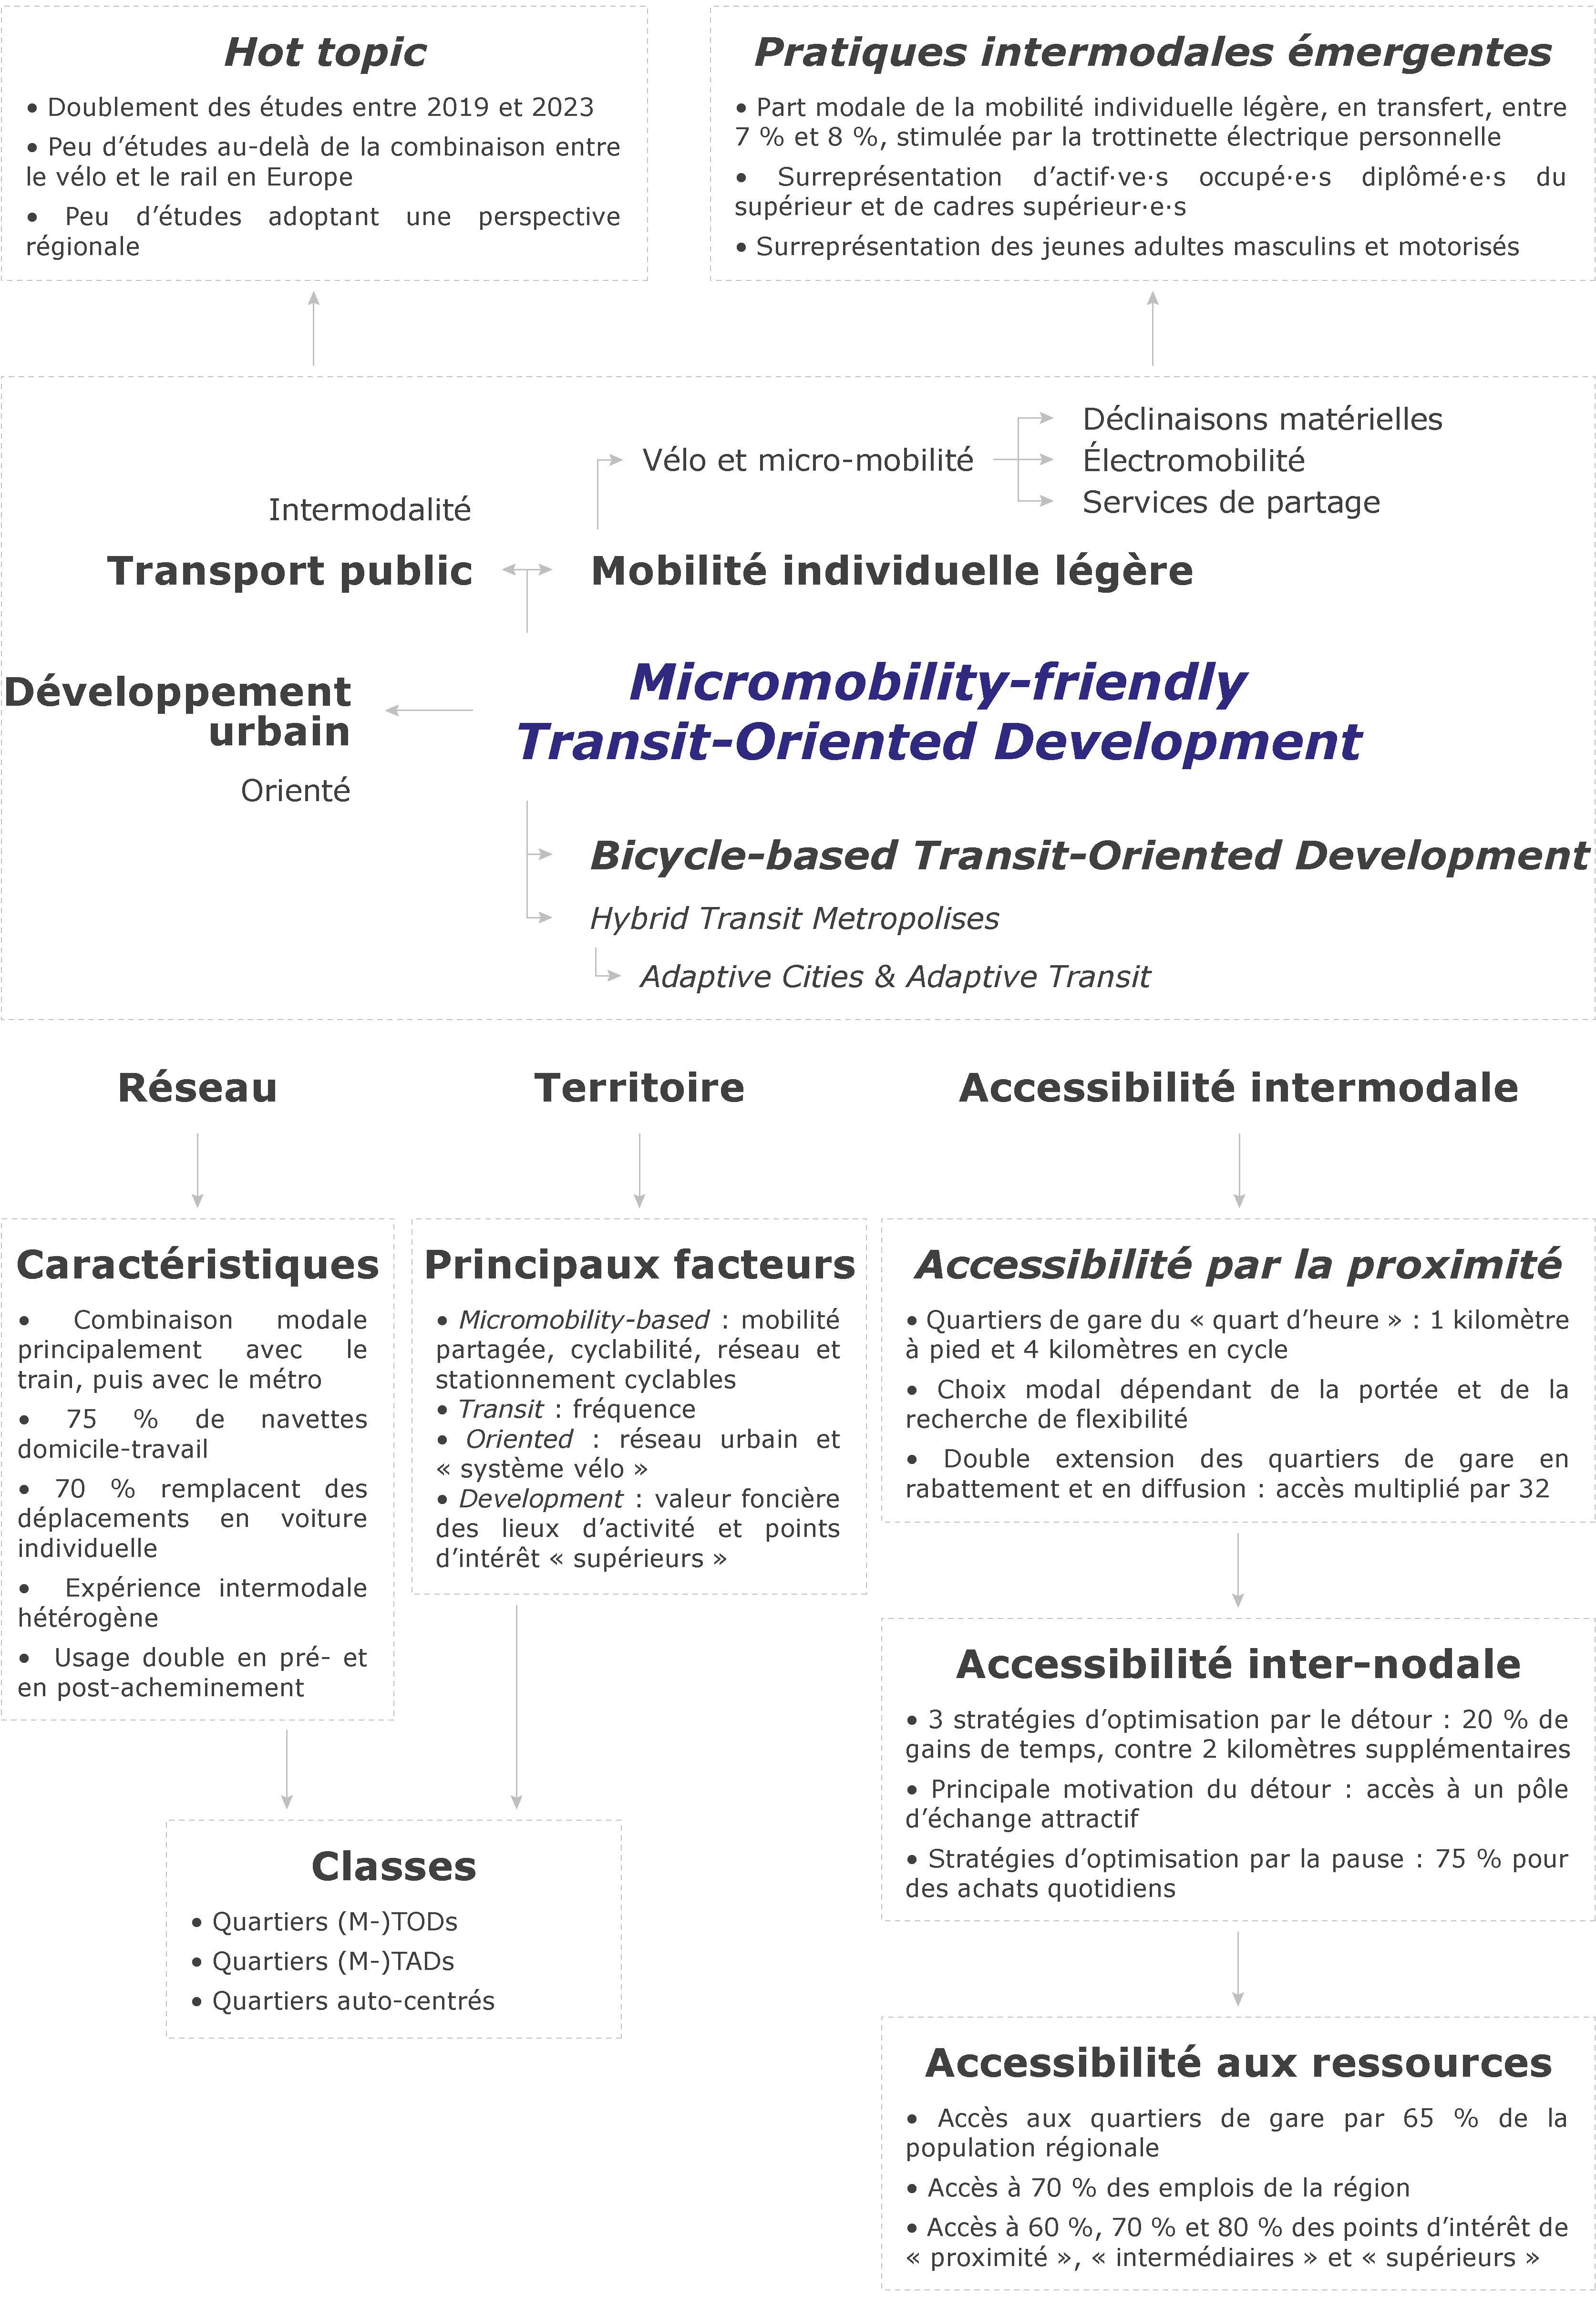
\includegraphics[width=1\columnwidth]{src/Figures/Conclusion/FR_Conclusion_generale.pdf}}
        \vspace{5pt}
        \begin{flushright}\scriptsize{
        Auteur~: \textcolor{blue}{Dylan Moinse (2025)}
        }\end{flushright}
    \end{figure}

% --- %
    \needspace{2\baselineskip} % Réserve de l'espace
\section*{Portée réflexive d'un \textsl{Micromobility-friendly Transit-Oriented Development}
    \label{conclusion-generale:portee-reflexive-mtod}
    }
    \addcontentsline{toc}{section}{Portée réflexive d'un \textsl{Micromobility-friendly Transit-Oriented Development}}
    %\markboth{Portée réflexive d'un \textsl{Micromobility-friendly Transit-Oriented Development}}{}
    \markright{Portée réflexive d'un \textsl{Micromobility-friendly Transit-Oriented Development}}{}

    % Introduction
L’objet de cette thèse a été de démontrer que l’intégration de la mobilité individuelle légère dans une conceptualisation d'un \acrfull{M-TOD} ne constitue pas une simple amélioration du \acrfull{TOD}, mais bien une transformation structurelle du modèle d’urbanisme orienté vers le rail. En adoptant une approche multi-niveaux, nous avons posé les bases d’un \acrshort{M-TOD}, intégrant la marche combinée et les pratiques intermodales, afin de redéfinir les proximités fonctionnelles des quartiers de gare. Sur le plan théorique, cette recherche s’inscrit dans une double filiation~: d’une part, elle prolonge les réflexions sur l’\Guillemets{urbanisme des réseaux} \textcolor{blue}{\autocite[]{dupuy_urbanisme_1991}}\index{Dupuy, Gabriel|pagebf}~; d’autre part, elle participe aux réflexions associées au \Guillemets{tournant de la mobilité}, en repositionnant la fabrique urbaine autour des proximités renouvelées \textcolor{blue}{\autocites{sheller_new_2006}[8]{sheller_mobilizing_2016}[13]{randell_no_2020}}\index{Sheller, Mimi|pagebf}\index{Urry, John|pagebf}\index{Randell, Richard|pagebf}. Dans cette perspective, les gares ne doivent plus être envisagées comme de simples points de connexion fonctionnels, mais bien comme des espaces intermodaux stratégiques, situés à l’interface du système urbain régional. Elles constituent des nœuds d’accessibilité, où la mobilité individuelle légère joue un rôle fondamental dans le maillage et l’extension des territoires rendus accessibles. Ces nouvelles pratiques de mobilité offrent la possibilité de dépasser une vision segmentée par mode de déplacement et strictement infrastructurelle du transport public, en améliorant la \Guillemets{la capacité relationnelle des réseaux} \textcolor{blue}{\autocite[15]{richer_quelles_2016}}\index{Richer, Cyprien|pagebf}\index{Meissonnier, Joël|pagebf}\index{Rabaud, Mathieu|pagebf} à partir d'une approche systémique \Guillemets{porte-à-porte}. De ce point de vue, l’\Guillemets{altermobilité} devient indissociable de la \gls{multimodalité} et de l’intermodalité \textcolor{blue}{\autocite[91-92]{vincent-geslin__2012}}\index{Vincent-Geslin, Stéphanie|pagebf}, favorisant une approche contextualisée du \acrshort{TOD}. Un changement de référentiel s’impose, en passant d'une logique d'attractivité à une \Guillemets{hospitalité} territoriale \textcolor{blue}{\autocite[2]{talandier_lhospitalite_2023}}\index{Talandier, Magali|pagebf}, qui engage une reconfiguration des stratégies urbaines en fonction des relations de proximité et des attentes en matière de cadre de vie, ouvrant la voie à une nouvelle manière de concevoir les interactions entre urbanisme et mobilité.%%Rédigé%%

    % Accessibilité
L’évaluation des seuils de distance et des aires d’influence associées aux itinéraires reliant les arrêts de transport en commun a permis de mettre en évidence une amélioration conjointe de l’accessibilité locale et régionale, résultant des pratiques intermodales. L’intégration de la mobilité individuelle légère favorise ainsi une meilleure connexion entre les quartiers de gare et le système ferroviaire, tout en élargissant les opportunités d’accès à l’échelle régionale. Au-delà de l’analyse des distances physiques, cette recherche doctorale s'est attachée à intégrer l'une des définitions les plus complètes de l'accessibilité \textcolor{blue}{\autocite[3]{chapelon_accessibilite_2006}}\index{Chapelon, Laurent|pagebf}, reposant sur quatre dimensions clés~: (i) la distribution géographique de l'offre et de la demande de ressources, (ii) la performance des réseaux, (iii) la temporalité et les rythmes, ainsi que (iv) les caractéristiques individuelles des usager·ère·s \textcolor{blue}{\autocite[128]{geurs_accessibility_2004}}\index{Geurs, Karst~T.|pagebf}\index{Wee, Bert van|pagebf}. L’objectif était alors d’évaluer comment la mobilité individuelle légère contribue à améliorer l'accessibilité intermodale, entendue à la fois comme une forme d'accessibilité \Guillemets{par la proximité} \textcolor{blue}{\autocite[2]{silva_proximity-centred_2023}}\index{Silva, Cecília|pagebf}\index{Büttner, Benjamin|pagebf}\index{Seisenberger, Sebastian|pagebf}\index{Rauli, Anna|pagebf}~; une accessibilité \Guillemets{nodale} \textcolor{blue}{\autocite[283-343]{chapelon_offre_1997}}\index{Chapelon, Laurent|pagebf}\index{Mathis, Philippe|pagebf}, mais aussi inter-nodale~; et une accessibilité aux ressources et aux destinations. Ce changement de paradigme positionne ainsi l’accessibilité non plus comme un simple outil de facilitation des déplacements, mais comme un levier de promotion de la proximité et de réorganisation des territoires \textcolor{blue}{\autocite[4]{levine_century_2020}}\index{Levine, Jonathan|pagebf}. Ce travail doctoral a montré que la mobilité individuelle légère permet de ce fait de renforcer les connexions entre les lieux d'intérêt à une échelle régionale, tout en favorisant un retour à un rythme urbain assimilé à celui de la \Guillemets{lenteur} \textcolor{blue}{\autocite[9]{silva_proximity-centred_2023}}\index{Silva, Cecília|pagebf}\index{Büttner, Benjamin|pagebf}\index{Seisenberger, Sebastian|pagebf}\index{Rauli, Anna|pagebf}. En somme, la complémentarité entre le transport public, la marche combinée et la mobilité individuelle légère se révèle encore largement sous-estimée dans les politiques de transport et d’aménagement, d'après \textcolor{blue}{Claude} \textcolor{blue}{\textcite[6-7]{soulas_triptyque_2021}}\index{Soulas, Claude|pagebf}, chercheur devenu expert indépendant, pour qui le développement de la marche combinée et du vélo est à même d'optimiser les réseaux de transport en commun de trois manières~:
\begin{customitemize}
    \item Tout d’abord, la mobilité individuelle légère permet de compenser l’hétérogénéité de la charge des lignes, en désaturant les tronçons centraux tout en rendant les extrémités des réseaux plus attractives. Cela limite ainsi le recours aux parcs relais automobiles, en offrant des alternatives viables pour accéder aux pôles d’échange~;
    \item Ensuite, l’intégration des cycles conduit à remettre en question les distances inter-stations, historiquement calibrées pour optimiser la desserte locale, mais qui contribuent paradoxalement à réduire la vitesse commerciale du réseau~;
    \item Enfin, ces synergies modales permettent une conception plus linéaire des lignes de transport public, en limitant la sinuosité des tracés à destination des pôles générateurs, qui contraint souvent les performances du réseau.
\end{customitemize}%%Rédigé%%

    % Vélomobilité
Dans la mesure où les aménagements cyclables privilégiés par les cyclistes, tels que les pistes cyclables, bandes cyclables et voies vertes, permettent d’allonger la longueur des itinéraires en améliorant le confort et la sécurité des déplacements \textcolor{blue}{\autocite{poisson_amenagements_2019}}\index{Poisson, Adrien|pagebf}\index{Chapelon, Laurent|pagebf}\index{Lammoglia, Adrien|pagebf}, le développement d'un système urbain conjugué à un \Guillemets{système vélo} stratégiquement orientés vers les réseaux de transport en commun s’imposent comme des leviers structurants pour concilier déplacements de proximité soutenables et connexions avec les pôles d’échange. Plus généralement, cette réflexion nous amène à considérer la \Guillemets{vélomobilité}, notion analogue à celle de l’\Guillemets{automobilité}, qui distingue trois dimensions en interaction \textcolor{blue}{\autocite[20-21]{rerat_au_2019}}\index{Rérat, Patrick|pagebf}~: les \textsl{usages} qui renvoie aux caractéristiques socio-démographiques et aux déplacements~; le \textsl{potentiel de mobilité cycliste} qui renvoie à l'accès au vélo, aux compétences, aux motivations et aux représentations sociales~; et le \textsl{potentiel d'accueil des territoires} qui renvoie à leur cyclabilité ainsi qu'aux normes et aux politiques. Selon \textcolor{blue}{Matt} \textcolor{blue}{\textcite[492]{watson_how_2012}}\index{Watson, Matt|pagebf}, chercheur et professeur à l'Université de Sheffield, les systèmes de \Guillemets{vélomobilité} et d'\Guillemets{automobilité} entrent en rivalité directe pour l’accès aux mêmes ressources, tant matérielles que symboliques. En d’autres termes, le développement d’un réseau cyclable structuré et connecté suppose une reconfiguration des infrastructures urbaines, souvent marquées par une hiérarchisation favorable aux véhicules motorisés. Ce phénomène s’illustre notamment dans les quartiers de gare, où la présence massive d’infrastructures dédiées à l’automobile constitue un frein à l’essor du vélo en rabattement vers les pôles de transport public. Finalement, la proportion relativement faible des déplacements intermodaux observée aujourd’hui ne doit pas masquer leur fort potentiel de développement, notamment en raison de la capacité de la mobilité individuelle légère à capter le report modal des automobilistes dans les territoires périurbains \textcolor{blue}{\autocite[22]{ulles_quelle_2024}}\index{Ullès, Jean-Clément|pagebf}\index{Chapelon, Laurent|pagebf}. Alors même qu'une \Guillemets{culture d’indifférence vis-à-vis du transport public} (\textsl{culture of indifference towards public transport}) subsiste et continue de prévaloir \textcolor{blue}{\autocite[656]{tan_identifying_2014}}\index{Tan, Wendy|pagebf}\index{Bertolini, Luca|pagebf}\index{Janssen-Jansen, Leonie|pagebf} dans ces contextes urbains, constituant un obstacle à une vision intégrée des déplacements. Dans cette optique, l’opérationnalisation du \acrshort{M-TOD} repose sur des leviers d’action concrets, qui doivent être activés par les acteurs de l’aménagement et des transports afin d’accélérer la transition vers un urbanisme ferroviaire à même de répondre aux enjeux régionaux actuels.%%Rédigé%%

% --- %
    \needspace{1\baselineskip} % Réserve de l'espace
\section*{Implications de la recherche doctorale
    \label{conclusion-generale:implications}
    }
    \addcontentsline{toc}{section}{Implications de la recherche doctorale}
    %\markboth{Implications de la recherche doctorale}{}
    \markright{Implications de la recherche doctorale}{}

    % Introduction
Dans la continuité des enseignements dégagés, nous avons souhaité formuler diverses recommandations à destination des acteurs de la fabrique urbaine, en appui aux politiques publiques en matière d'aménagement et de transport. Ces préconisations n'ont pas vocation à être exhaustives, ni à proposer un niveau de précision permettant leur intégration immédiate dans les orientations stratégiques. Elles s'apparentent davantage à des principes, à l'image d'un manifeste, visant à inspirer de nouvelles approches et méthodes et à offrir des pistes de réflexion transposables selon les contextes. Ces recommandations, sous forme de volets, s’inscrivent dans une logique d’activation des leviers de transition, en proposant des axes d’action stratégiques pour favoriser l’intégration de la mobilité individuelle légère dans les quartiers de gare et renforcer l’intermodalité au sein des réseaux de transport public. Les orientations que nous suggérons se déclinent en dix volets distincts, intégrant un éventail de mesures et d’initiatives possibles, détaillées ci-après.%%Rédigé%%

    \needspace{1\baselineskip} % Réserve de l'espace
\subsubsection*{Pistes stratégiques et organisationnelles
    \label{conclusion-generale:implications-gouvernance}
    }

% Documents d'urbanisme
    \begin{displayquote}
\textbf{Volet 1~: Inscrire les quartiers de gare comme des lieux stratégiques au cœur des orientations stratégiques de développement territorial.}
\\
\textsl{Intégrer et réévaluer les périmètres fonctionnels des quartiers de gare dans les référentiels stratégiques d’aménagement et de mobilité.}
    \end{displayquote}
L'enjeu du premier volet des recommandations est de redéfinir les périmètres étendus des quartiers de gare dans les plans d’aménagement et de mobilité, afin de dépasser les limites d’une planification centrée exclusivement sur la proximité immédiate des pôles d’échange. Actuellement, la plupart des stratégies d’urbanisme et de transport continuent de considérer les quartiers de gare selon des périmètres restreints, souvent définis à l’échelle de l’accessibilité piétonne traditionnelle, négligeant ainsi le potentiel d’extension permis par la valorisation de la \gls{marchabilité} et de la cyclabilité. Cette approche implique une révision des documents d’urbanisme et des plans de mobilité~–~le \acrfull{SCoT} comme le \acrfull{PLU} ou le \acrfull{PDM}~–, afin d’adapter les cadres réglementaires et opérationnels aux quartiers de gare étendus. En mobilisant les outils de mesure et de représentation cartographique développés dans cette recherche, il devient possible de repenser le zonage autour des pôles d’échange, en tenant compte des aires d’influence réelles des gares.%%Rédigé%%

% Observatoire
    \begin{displayquote}
\textbf{Volet 2~: Faire des quartiers de gare des laboratoires d’innovation urbaine et de nouvelles pratiques d’aménagement.}
\\
\textsl{Mettre en place un observatoire de l'urbanisme orienté vers les transports en commun et de l'intermodalité, destiné à évaluer les initiatives et les expérimentations.}
    \end{displayquote}
L'enjeu du deuxième volet réside dans le développement d'organismes dédiés à l’étude des interactions entre urbanisme et mobilité, avec une focale intermodale, inscrivant ainsi les quartiers de gare dans une dynamique d’expérimentation et d’évaluation continue. Dans une perspective de diffusion et de transférabilité des \Guillemets{bonnes pratiques}, ces observatoires constitueraient des instruments d’analyse permettant de mesurer l’évolution des pratiques intermodales, d’évaluer les expérimentations en matière de rabattement et de cadre urbain, mais aussi d’adapter l'appui aux politiques publiques en fonction des résultats empiriques obtenus. Au-delà de leur rôle de veille, d’évaluation et de comparaison entre territoires, ces dispositifs offriraient un cadre méthodologique structurant pour tester et comparer différentes configurations d’intégration de la mobilité individuelle légère dans les pôles d’échange, à travers des expérimentations en zones pilotes, tout en recueillant des données utiles. Ils contribueraient ainsi à une meilleure compréhension des facteurs influençant l’adoption des pratiques intermodales et permettraient d’anticiper les tendances émergentes en matière de mobilité et d’aménagement des territoires ferroviaires. L’opérationnalisation d'une telle structure transversale supposerait une collaboration étroite entre collectivités locales, opérateurs de transport, chercheur·se·s, associations, ainsi que les usager·ère·s elleux-mêmes, en vue d'une prise de décision éclairée.%%Rédigé%%

    \needspace{1\baselineskip} % Réserve de l'espace
\subsubsection*{Lignes d'action pour favoriser l'intermodalité
    \label{conclusion-generale:implications-mobilites}
    }

% Information voyageurs
    \begin{displayquote}
\textbf{Volet 3~: Déployer des outils d’information et de communication dédiés à l’intermodalité.}
\\
\textsl{Améliorer l'accès à l'information et sensibiliser aux bénéfices de l'usage intermodal de la mobilité individuelle légère.}
    \end{displayquote}
Le troisième volet des recommandations porte sur l’amélioration de l’information, de la communication et de la sensibilisation autour des parcours intermodaux impliquant la mobilité individuelle légère. Nous préconisons de développer des algorithmes couplés à des cartographies dynamiques, accessibles à la fois physiquement dans les gares et dans les espaces publics, et numériquement via des applications mobiles et des plate-formes en ligne. Ces outils interactifs permettraient aux usager·ère·s potentiel·le·s d’identifier en temps réel les infrastructures et les services facilitant l’intermodalité, comme les itinéraires cyclables sécurisés, les espaces de stationnement vélo, les services de partage ou encore les connexions intermodales qu'il est possible d'optimiser. En intégrant des fonctionnalités de navigation multimodale, à la manière du \acrshort{MaaS}, ces applications offriraient des suggestions d’itinéraires optimisés, prenant en compte les préférences des utilisateur·rice·s ou encore la disponibilité des services de location et de stationnement sécurisé. Parallèlement, une stratégie de communication ciblée, tout comme le recours à la \Guillemets{gamification}, permettrait d’encourager l’adoption de ces pratiques intermodales, en mettant en avant les bénéfices de la mobilité individuelle légère dans le cadre d'un rabattement vers les gares. Des campagnes de sensibilisation, sous forme d’actions locales, d’événements de promotion et de partenariats avec les acteurs du transport et de l’aménagement, contribueraient à lever les freins cognitifs et culturels associés à ces nouvelles pratiques. Il s’agirait ainsi de créer un environnement propice à l’intermodalité, où l’accessibilité à l’information et la valorisation des alternatives à la voiture individuelle jouent un rôle clé dans le changement des comportements.%%Rédigé%%

% Mobilité partagée
    \begin{displayquote}
\textbf{Volet 4~: Développer un réseau de services de mobilité partagée à l'échelle nationale ou régionale, avec un maillage stratégique des pôles d'échange et des quartiers de gare.}
\\
\textsl{Renforcer l’intermodalité en développant un réseau national ou régional de services de mobilité partagée au sein des aires d'influence des lieux d'échange.}
    \end{displayquote}
Le quatrième volet des recommandations s’inscrit dans une logique de complémentarité modale et de renforcement de la visibilité de la mobilité individuelle légère dans l’espace urbain. Il propose de développer un réseau de services de vélo et, ou bien, de trottinette en libre-service, déployé de manière stratégique autour des pôles d’échange, afin de faciliter l’intermodalité et d’étendre les possibilités de rabattement vers les gares. L’enjeu principal est d’intégrer une offre de location de courte et de longue durée, accessible aussi bien pour des usages occasionnels que pour des déplacements quotidiens. Cela passe par le développement d'une flotte de véhicules partagés, électriques ou non, opérée par un acteur à une échelle géographique pertinente avec le système intermodal\footnote{
    La mise en œuvre d'un tel service de mobilité, par un opérateur public ou privé, ne peut éviter de poser la question du modèle d'affaire (\Guillemets{business model}) associé qui reste à définir.
}, c’est-à-dire au niveau régional ou national, à l'instar des expériences néerlandaises ou belges, plutôt que selon des périmètres métropolitains ou communaux cloisonnés. La réussite d’un tel dispositif repose sur la mise en place d’un maillage dense de stations de dépose, situées non seulement au sein et autour des gares, mais également dans les quartiers de gare étendus, là où les besoins de rabattement sont les plus importants. Afin d’optimiser l’usage de ces services et de renforcer leur attractivité, il est essentiel d’accompagner ce déploiement par une billettique intégrée, permettant d’accéder aussi bien aux systèmes de transport en commun qu’aux services de mobilité partagée par le biais d'un titre unique. Cette billettique unifiée pourrait être couplée à des incitations tarifaires, par exemple en offrant des réductions aux abonné·e·s du transport public. À ce titre, cette orientation entre en résonance avec les ambitions régionales formulées dans le principe 18 du Plan Vélo, présent dans le \acrfull{SRADDET} de la \textcolor{blue}{\textcite[40]{region_hauts-de-france_plan_2023}}\index{Région Hauts-de-France@\textsl{Région Hauts-de-France}|pagebf}. Cette suggestion mentionne explicitement la volonté de lancer une \Guillemets{\textsl{expérimentation de vélo libre-service à l’échelle d’un territoire ou d’une ligne de train.}}. Le rapport émis par le \textcolor{blue}{\textcite[75]{ceser_hauts-de-france_mobilite_2021}}\index{CESER Hauts-de-France@\textsl{CESER Hauts-de-France}|pagebf}\index{Bally, Stéphane|pagebf}\index{Melcus, Alain|pagebf} va également dans ce sens, même si cette structure met en avant l'intérêt d'un système de location à l'échelle régionale, plutôt que des services bigarrés.%%Rédigé%%

% Politique d'embarquement
    \begin{displayquote}
\textbf{Volet 5~: Mettre en place une politique d’emport de vélo et de trottinette axée sur les services ferroviaires express, en intégrant des espaces dédiés facilitant l’embarquement des véhicules les plus compacts.}
\\
\textsl{Favoriser l’intermodalité en facilitant l’embarquement du vélo et de la micro-mobilité à bord des services ferroviaires express.}
    \end{displayquote}
Le cinquième volet porte sur l’évolution des politiques d’emport du vélo et de la micro-mobilité à bord du train\footnote{
    L'hospitalité des territoires passe également par un meilleur accueil de la mobilité individuelle légère dans les transports en commun, mais peut-être aussi sur une forme de réciprocité entre ces véhicules et les infrastructures qui les accueillent. Certains faits divers illustrent les enjeux de cette cohabitation. Par exemple, en 2022, une \acrfull{TEP} a pris feu à bord d'un train en Espagne, conduisant les autorités régulatrices à interdire leur embarquement un an plus tard \textcolor{blue}{\autocite{cottrel_trottinette_2022}}\index{Cottrel, Olivier|pagebf}. Cet incident soulève des questions de sécurité, en particulier sur la qualité des batteries électriques. En ce sens, cet élément factuel rappelle combien il est essentiel d'impliquer des efforts de réglementation d'une part, et d'amélioration technique et d'usage d'autre part.
}, afin de faciliter la réalisation de déplacements intermodaux. Dans une logique d’optimisation des flux et dans la lignée de nos observations, il serait pertinent de cibler en priorité les trains express, plutôt que les services ferroviaires de type omnibus, pour l’aménagement de compartiments dédiés à l’emport de ces véhicules. Ces trains, en raison de leurs distances parcourues plus longues et de leur nombre d’arrêts limité, sont particulièrement stratégiques pour favoriser les déplacements intermodaux sur des territoires élargis, où l’association entre train et mobilité individuelle légère constitue une alternative crédible à l’usage de la voiture individuelle. Une attention particulière devrait être portée aux véhicules compacts et facilement transportables, tels que le vélo pliant et la \acrfull{TEP}, qui ne bénéficient actuellement d’aucun aménagement adapté dans la plupart des trains. Pourtant, ces véhicules sont particulièrement adaptés aux logiques intermodales. L’intégration d’espaces spécifiques à ces équipements permettrait donc d’améliorer le confort et la fluidité des déplacements intermodaux, tout en renforçant leur compétitivité face à l’usage exclusif de l’automobile. En cela, l'aménagement de compartiments modulables, adaptés au type de véhicule dans les voitures, constituerait une forme d'innovation intéressante.%%Rédigé%%

% Politique de stationnement
    \begin{displayquote}
\textbf{Volet 6~: Renforcer l’offre de stationnement sécurisé aux abords des pôles d’échange et dans les quartiers de gare, en veillant à une capacité et à un accès attractifs, ainsi qu'à une adaptation au type de véhicule.}
\\
\textsl{Développer, au sein des quartiers de gare étendus, des infrastructures de stationnement sécurisées, accessibles et adaptées à la diversification de la mobilité individuelle légère.}
    \end{displayquote}
Le sixième volet des recommandations s'attache au développement d’infrastructures de stationnement adaptées aux cycles, afin de faciliter l’adoption intermodale de la mobilité individuelle légère et de renforcer l’attractivité des réseaux de transport en commun. L’un des principaux freins à l’usage combiné du vélo et du train réside dans le manque d’espaces sécurisés et adaptés pour le stationnement des véhicules. Pour répondre à cet enjeu, il est nécessaire d’installer des infrastructures de stationnement sécurisées, non seulement à proximité immédiate des gares, mais aussi dans les quartiers de gare étendus, où les besoins de rabattement sont particulièrement importants. Ces espaces doivent être conçus pour accueillir une diversité de véhicules. Ces infrastructures pourraient également intégrer des bornes de recharge pour les modes de déplacement électriques ou assistés. De même, la mise en place de consignes sécurisées pour les véhicules les plus compacts offrirait une solution complémentaire pour encourager leur usage dans le cadre de déplacements intermodaux. Si, dans les grandes gares métropolitaines, les vélostations capacitaires tendent à émerger, sous l'effet de la \acrfull{LOM}, les gares secondaires pourraient quant à elles bénéficier d'espaces de stationnement mutualisés ou de consignes individuelles. L’accessibilité de ces stationnements doit être pensée de manière à faciliter leur usage quotidien, en garantissant soit un accès libre et ouvert dans l’\gls{espace public}, soit une interopérabilité avec les systèmes de transport en commun. Un principe d’accès intégré, via un ticket de transport ou un abonnement, permettrait d’assurer une continuité de service et de renforcer l’attractivité du système intermodal. La mise en place de capteurs de suivi des flux permettrait d'adapter les infrastructures aux besoins en anticipant les extensions nécessaires.%%Rédigé%%

    \needspace{1\baselineskip} % Réserve de l'espace
\subsubsection*{Axes d'amélioration pour aménager les quartiers de gare
    \label{conclusion-generale:implications-amenagement}
    }

% Aménagements cyclables
    \begin{displayquote}
\textbf{Volet 7~: Renforcer la connectivité des quartiers de gare grâce à un réseau cyclable structurant, qualitatif et sécurisé.}
\\
\textsl{Structurer un réseau intercommunal cyclable pour étendre et améliorer l'accès aux gares.}
    \end{displayquote}
Développer un maillage intercommunal d’itinéraires cyclables continus et sécurisés, reliant les quartiers de gare étendus aux gares ferroviaires, mais également les quartiers de gare entre eux, représente le septième volet. Cet objectif se traduit par le renforcement de la connectivité cyclable, en garantissant des infrastructures directes, sécurisées et confortables, tout en corrigeant ou en traitant les coupures urbaines. Il s'agit, dans le même intérêt, d'accorder une priorité aux continuités piétonnes et cyclables, notamment le long des voies structurantes \textsl{au sein} et \textsl{entre} les quartiers de gare, afin de créer des liaisons entre les gares permettant alors de renforcer la capillarité du réseau de transport en commun. L’objectif est ainsi d’assurer un système de rabattement performant, basé d'abord sur les axes majeurs connectés aux nœuds de transport en commun, sur les intersections et structurant les voies secondaires. Pour structurer et hiérarchiser ce réseau cyclable, la mise en cohérence des itinéraires sous forme d’\Guillemets{autoroutes à vélo} ou d'un projet fédérateur de \Guillemets{\acrshort{RER} vélo} constituerait une avancée majeure. Ces réseaux cyclables stratégiques permettraient d’identifier les corridors les plus structurants et de favoriser une planification intégrée du réseau cyclable à l’échelle régionale. Ce dispositif devrait également s’accompagner d’un travail sur l’identité visuelle et la signalétique, afin de rendre le réseau plus identifiable et attractif pour les cyclo-voyageur·se·s et les cyclistes. L’installation d’une signalétique claire et homogène, couplée à des services dédiés, tels que des aires de repos, des bornes de réparation ou encore des stations de recharge électrique, contribuerait à rendre ces itinéraires plus accessibles et fonctionnels. Ces recommandations s’inscrivent dans les recommandations d'orientation stratégique déjà formulées à l’échelle régionale. Le rapport du \textcolor{blue}{\textcite[72]{ceser_hauts-de-france_mobilite_2021}}\index{CESER Hauts-de-France@\textsl{CESER Hauts-de-France}|pagebf}\index{Bally, Stéphane|pagebf}\index{Melcus, Alain|pagebf}, portant sur le développement territorial régional, préconise en effet la construction d’un réseau intercommunal cyclable, avec parmi ses objectifs principaux le rabattement vers les gares en complément des infrastructures de location et de stationnement vélo.%%Rédigé%%

% Contraindre l'automobile
    \begin{displayquote}
\textbf{Volet 8~: Réduire la place de l'automobile dans les quartiers de gare.}
\\
\textsl{Rééquilibrer le partage de l’espace public en limitant l’usage de la voiture dans les quartiers de gare.}
    \end{displayquote}
Le huitième volet des recommandations s’inscrit dans une approche coercitive de l’aménagement du territoire, fondée sur les résultats de cette recherche quant à la compétitivité de l’intermodalité face à l’automobile. Nos analyses montrent en effet que l’intermodalité ne devient véritablement compétitive que lorsque l’environnement urbain impose des contraintes à l’usage de la voiture individuelle. Il s’agit d’agir simultanément sur plusieurs leviers afin de limiter l’usage de l'\Guillemets{autosolisme}. La première mesure concerne la réduction de la circulation automobile, en agissant sur le trafic et la vitesse dans les périmètres des gares. En instaurant des zones apaisées, où la circulation est restreinte ou limitée à des vitesses réduites, il devient possible de rééquilibrer l’espace public au profit de la marche et des cycles. Cette initiative doit être accompagnée de piétonisations dans certaines voies structurantes permettant de créer des parcours confortables à destination des gares. En complément, la réduction progressive des espaces de stationnement automobile au sein des quartiers de gare constitue un levier stratégique pour dissuader l’usage systématique de la voiture individuelle. Il ne s’agit pas d’éliminer ces équipements, mais d’adapter leur nombre et leur gestion, afin de privilégier des solutions alternatives telles que les parcs relais, mutualisés ou encore les espaces réservés au covoiturage et aux véhicules partagés. En parallèle, l’introduction de mesures de tarification désincitative du stationnement pourrait constituer un levier efficace pour orienter les choix modaux. La mise en place d’une tarification différenciée, en fonction de la durée de stationnement ou de la situation personnelle, permettrait d’encourager les automobilistes à privilégier d’autres solutions de déplacement.%%Rédigé%%

    \needspace{1\baselineskip} % Réserve de l'espace
\subsubsection*{Propositions pour une planification intégrée à l'échelle régionale
    \label{conclusion-generale:implications-planification}
    }

% Urbanisme
    \begin{displayquote}
\textbf{Volet 9~: Intervenir sur les activités et sur le bâti afin de densifier et de diversifier les usages.}
\\
\textsl{Adapter les formes urbaines et les activités pour un urbanisme du \Guillemets{Quart d'Heure}.}
    \end{displayquote}
Ce neuvième volet suppose des mesures de densification et de diversification des activités urbaines, de sorte à reconfigurer les formes urbaines, les rythmes urbains et les proximités dans les quartiers de gare. L’un des objectifs est de concentrer et de distribuer plus efficacement les fonctions résidentielles, commerciales et autres autour des pôles d’échange, de manière à favoriser une urbanisation plus équilibrée et une intensification des usages à proximité des gares. Il ne s’agit pas seulement d’accroître la densité bâtie, mais surtout de favoriser une diversité des fonctions urbaines qui garantisse une meilleure répartition des flux. L’enjeu central de ce volet est ainsi de repenser la fabrique urbaine des quartiers de gare sous l’angle du principe du \Guillemets{Quart d’Heure}. L’idée est d’adopter une approche qui permette à chaque résident·e ou usager·ère d’accéder aux principales aménités urbaines en moins de quinze minutes, que ce soit à pied, en cycle ou en transport public. Une telle refonte implique une révision des règlements d’urbanisme et des outils de planification territoriale pour inciter à la construction de logements à proximité des gares, en garantissant une répartition équilibrée des types d’habitat. En définitive, ce neuvième volet appelle à une transformation profonde et systémique des politiques d’urbanisme et de transport, en plaçant la proximité, l’accessibilité et l’intermodalité au cœur des stratégies de planification.%%Rédigé%%

% Artificialisation
    \begin{displayquote}
\textbf{Volet 10~: Encadrer l'artificialisation des sols pour préserver les ressources foncières.}
\\
\textsl{Mettre en œuvre une politique systémique de sobriété foncière en lien avec le \acrshort{M-TOD}.}
    \end{displayquote}
La limitation de l’artificialisation des sols constitue un enjeu majeur de long terme, comme en témoigne ce dixième volet des recommandations. L’objectif est d’éviter un étalement urbain excessif et de préserver les espaces naturels et agricoles situés en périphérie des quartiers de gare, tout en garantissant une urbanisation maîtrisée et soutenable. Dans cette perspective, l’urbanisation des zones ferroviaires doit être pensée en priorité à partir des espaces déjà artificialisés, en favorisant la réhabilitation des friches urbaines et la densification des secteurs bâtis plutôt que l’extension urbaine non maîtrisée. L’enjeu est ainsi de concilier croissance urbaine et sobriété foncière, en accord avec les politiques publiques récentes de ralentissement et de compensation, issus de l'objectif de \acrfull{ZAN}. Les stratégies urbaines à long terme impliquent ainsi la question de la maîtrise foncière, qui peuvent être pensées à travers la mise en place d'une trame verte et bleue en coordination avec le modèle de développement urbain. Cette démarche s’inscrit dans une volonté de renforcer la qualité de vie en réduisant les îlots de chaleur urbains, en améliorant le cadre paysager. La présence de végétation, de plans d’eau et d’espaces récréatifs à proximité des infrastructures de transport en commun favorise l’acceptabilité sociale des projets d’aménagement, tout en jouant un rôle clé dans l'amélioration de l'attractivité des réseaux de transport en commun et du cadre de vie. En définitive, ce dixième volet appelle à une planification urbaine résiliente et écologique, en combinant densification maîtrisée et en \Guillemets{construisant la ville sur la ville}.%%Rédigé%%

% --- %
    \needspace{1\baselineskip} % Réserve de l'espace
\section*{Prolongements et perspectives de recherche
    \label{conclusion-generale:perspectives}
    }
    \addcontentsline{toc}{section}{Perspectives de recherche}
    %\markboth{Perspectives de recherche}{}
    \markright{Perspectives de recherche}{}

    % Introduction
Si cette recherche a permis d’apporter des éléments conceptuels, méthodologiques et empiriques à ce sujet de recherche, certaines limites inhérentes à la démarche et aux terrains étudiés doivent être reconnues. Toute recherche s’inscrit effectivement dans un cadre méthodologique et temporel contraint, qui oriente l’analyse et conditionne les résultats obtenus. Cette dernière section vise ainsi à expliciter les limites de ce travail, tant du point de vue des données mobilisées, des méthodes employées que de la portée des conclusions, tout en avançant des pistes de recherche futures susceptibles de prolonger et d’approfondir ces réflexions. En miroir de ces limites, cette réflexion sur les limites et prolongements possibles permet ainsi d’identifier les champs d’investigation complémentaires qui pourraient être explorés par la recherche académique et les acteurs opérationnels, afin d’affiner, d'améliorer et d’adapter le modèle \acrshort{M-TOD} aux contextes.

    \needspace{1\baselineskip} % Réserve de l'espace
\subsubsection*{Approfondissements conceptuels
    \label{conclusion-generale:perspectives-pistes-theoriques}
    }

    % Proximité
Sur le plan conceptuel, l’intégration de la mobilité individuelle légère au sein du \acrshort{M-TOD} conduit à une réinterrogation de la notion de proximité, en l’articulant avec d’autres courants émergents en urbanisme et en aménagement du territoire. Si le concept renouvelé de la \Guillemets{Ville du Quart d’Heure} a été largement mobilisé dans cette recherche, c’est en raison de sa complémentarité avérée avec le \acrshort{TOD} et le \acrshort{M-TOD}, une relation désormais reconnue au sein d’une large communauté scientifique. À cet égard, plusieurs démarches ont récemment contribué à affiner cette articulation, notamment à travers les \textsl{Transit-Oriented Development-based 15-minute cities}, qui soulignent la compatibilité et les synergies entre ces deux modèles d’aménagement \textcolor{blue}{\autocite[11]{wolanski_potential_2023}}\index{Wolański, Michał|pagebf}. Ces réflexions s’inscrivent plus largement dans une approche centrée sur l’expérience des usager·ère·s et la qualité urbaine, à l’instar du \textsl{People-Oriented Development}, qui vise à replacer les dimensions sociales et territoriales au cœur des stratégies d’urbanisme et de transport. Ce concept participe ainsi à une réflexion élargie sur les proximités et les interactions entre infrastructures et pratiques de mobilité, et constitue à ce titre une piste féconde pour renouveler l’approche de la planification urbaine \textcolor{blue}{\autocite{davis_people_2024}}\index{Davis, Michael Maks|pagebf}\index{Verlinghieri, Ersilia|pagebf}. Enfin, une évolution encore plus récente dans le débat académique mérite, à nos yeux, d’être mentionnée~: le \textsl{Proximity-Oriented Development}, qui tend à faire dialoguer le \acrshort{TOD} avec les proximités territoriales et les géoproximités. Il s'agit notamment d'approfondir la notion de proximité, en ne la considérant plus seulement comme une simple ressource territoriale, mais en l'articulant avec la \Guillemets{proxibilité}, entendue comme un actif territorial \textcolor{blue}{\autocite{lebrun_proximite_2024}}\index{Lebrun, Nicolas|pagebf}. Ce cadre conceptuel, bien qu’encore en cours de formalisation, offre une perspective stimulante pour cette recherche doctorale, en prolongeant la réflexion sur l’intégration de la mobilité individuelle légère \textcolor{blue}{\autocite[3]{plastara_15-minute_2023}}\index{Plastara, Dimitra|pagebf}\index{Pozoukidou, Georgia|pagebf}.%%Rédigé%%

    % Cycles comme un réseau
D’un point de vue plus pratique, il apparaît opportun d’aller plus loin dans le questionnement sur les relations étroites entre le réseau de transport en commun et le réseau cyclable, en envisageant la notion de \Guillemets{système vélo} comme une composante à part entière d’un réseau de transport structurant. Cette perspective s’inscrit pleinement dans les dynamiques actuelles d’aménagement, notamment à travers les initiatives de \Guillemets{\acrshort{RER} vélo}, qui reprennent les principes de structuration des réseaux ferroviaires régionaux en proposant des \Guillemets{autoroutes à vélo}, caractérisées par des lignes identifiables et par des arrêts marquant des lieux d'intérêt et équipées d'équipements et de services. En matérialisant ainsi une organisation systémique des flux cyclables, ces infrastructures dépassent la simple conception du vélo comme mode individuel pour en faire un vecteur de mobilité territoriale, apte à structurer les déplacements quotidiens aux échelles métropolitaine et régionale. Dès lors, une piste de recherche stimulante consisterait à analyser le \Guillemets{système vélo} sous l’apparence d’un réseau de transport en commun à part entière, en questionnant dans quelle mesure il répond à des logiques similaires de maillage, de performance et d’interconnexion. À l’instar de la relation de connexion \Guillemets{naturelle} entre un réseau ferroviaire interurbain et un réseau ferroviaire urbain~–~comme celle existant entre le \acrshort{TER} et le métro~–, il s’agirait d’explorer les relations entre les nœuds des réseaux cyclables et les gares ferroviaires, dans une vision intégrée de la mobilité.%%Rédigé%%

    \needspace{1\baselineskip} % Réserve de l'espace
\subsubsection*{Pistes sur les méthodes et les outils d'analyse
    \label{conclusion-generale:perspectives-pistes-methodes}
    }

    % Quantitatif - limites
En considérant la méthodologie, la démarche adoptée présente certaines limites, d'abord en ce qui concerne la mobilisation des approches quantitatives~: la représentativité des échantillons et l’extrapolation des résultats en sont deux éléments représentatifs. L’échantillon des cyclo-voyageur·se·s étudié·e·s, constitué à partir de l'observation quantitative et du questionnaire, pourrait être élargi afin de mieux intégrer les populations sous-représentées et de tenir compte des spécificités de chaque type de véhicule relevant de la mobilité individuelle légère. Un autre biais méthodologique réside dans la focalisation sur l’usage effectif des combinaisons modales observées, au détriment d’une analyse des phénomènes de \Guillemets{non-usage}, c’est-à-dire des individus n’ayant pas adopté ces pratiques, mais présentant un potentiel de report modal. Cette limite concerne non seulement les \Guillemets{non-cyclistes}, mais également les \Guillemets{néocyclistes}, ainsi que les pratiques de \Guillemets{mésusage}, qui mériteraient une investigation plus approfondie. Enfin, la difficulté d’évaluer l’impact à long terme de l’intégration de la mobilité individuelle légère dans les stratégies \acrshort{TOD}\textcolor{blue}{s} constitue une autre faiblesse de la recherche doctorale. En ce sens qu'elle repose essentiellement sur des données statiques, captées à un instant donné, alors qu’une approche longitudinale permettrait d’appréhender l’évolution des pratiques intermodales et des transformations des quartiers de gare sur une période plus étendue.%%Rédigé%%

    % Quantitatif - pistes
Pour remédier à ces limites méthodologiques, plusieurs pistes d’amélioration peuvent être envisagées. Tout d’abord, une approche plus systématique du traitement de données massives permettrait de compenser les biais d’échantillonnage et d’affiner l’analyse des comportements intermodaux. L’exploitation des données issues de la \textsl{Big Data}, en intégrant notamment les données de fréquentation fournies par les opérateurs de transport et les tracés \acrshort{GPS} extraits des smartphones, offrirait une vision plus fine et dynamique des flux réalisés aussi bien avec un service de \acrshort{VLS}, de \acrshort{VFF}, de \acrshort{TEFF}, qu'avec un vélo ou un engin personnel. S'agissant des outils d'analyse, l’enjeu serait de développer des scénarios prospectifs, en s’appuyant sur des modélisations multi-agents, désormais envisageables grâce aux premiers enseignements recueillis sur les comportements \Guillemets{types} des usager·ère·s. L’adoption d’une approche \Guillemets{microscopique}, mobilisant des outils avancés tels que le projet \textsl{open source} \acrfull{MATSim}, permettrait de simuler les comportements de mobilité individuels, en tenant compte des caractéristiques propres des voyageur·se·s et de divers scénarios prospectifs, tout en réintégrant ces comportements dans le cadre de leur affectation au réseau de transport \textcolor{blue}{\autocite[119]{chapelon_transports_2016}}\index{Chapelon, Laurent|pagebf}. Une telle démarche présenterait l’avantage de mieux appréhender la population des \Guillemets{non-cyclistes}, qui demeure souvent marginalisée dans les études actuelles \textcolor{blue}{\autocite{poisson_amenagements_2019}}\index{Poisson, Adrien|pagebf}\index{Chapelon, Laurent|pagebf}\index{Lammoglia, Adrien|pagebf}.%%Rédigé%%
    
    % Qualitatif - limites
Dans l'esprit d'une échelle d'analyse \Guillemets{microscopique} avec un regard plus qualitatif, la démarche \Guillemets{macro-spatiale} adoptée dans cette thèse, et basée sur l’interaction entre réseau et territoire à l’échelle régionale, implique certaines limites quant à la prise en compte des dynamiques socio-spatiales à des échelles plus fines. En effet, cette recherche ne prétend pas englober l’ensemble des facteurs explicatifs des pratiques de mobilité, notamment en ce qui concerne les échelles \Guillemets{méso-} et \Guillemets{micro-spatiales}, où se jouent des ajustements plus subtils dans les usages et les stratégies modales \textcolor{blue}{\autocite[7]{desjeux_sciences_2004}}\index{Desjeux, Dominique|pagebf}. Certes, la réalisation exploratoire de parcours commentés constitue une première approche \Guillemets{nano-sociologique}, en intégrant les dimensions normatives, inconscientes et affectives des comportements de mobilité \textcolor{blue}{\autocite[7]{desjeux_sciences_2004}}\index{Desjeux, Dominique|pagebf}. Toutefois, ces enquêtes qualitatives, bien qu’essentielles, restent limitées en nombre et gagneraient à être étendues et diversifiées afin d’embrasser une pluralité de contextes et de profils d’utilisateur·rice·s. Par ailleurs, l’attention portée aux dimensions urbanistiques dans cette recherche, bien qu’indispensable pour comprendre les configurations spatiales de la mobilité intermodale, ne saurait, à elle seule, expliquer l’ensemble des dynamiques sociales qui structurent les pratiques intermodales \textcolor{blue}{\autocite[4]{gaudron-arlon_gender_2022}}\index{Gaudron-Arlon, Léa|pagebf}. Il apparaît donc essentiel d’adopter une approche pluridimensionnelle, croisant les enjeux spatiaux, sociaux et individuels, afin de restituer la complexité des chaînes de déplacement \textcolor{blue}{\autocite[7]{heesch_gender_2012}}\index{Heesch, Kristiann~C.|pagebf}\index{Sahlqvist, Shannon|pagebf}\index{Garrard, Jan|pagebf}.%%Rédigé%%

    % Qualitatif - pistes
Pour approfondir ces dimensions qualitatives, plusieurs pistes de recherche peuvent être envisagées. L'une d'entre elles consisterait à mobiliser le concept de \Guillemets{motilité}, conçu comme un capital de mobilité, qui reflète l’articulation entre les opportunités de déplacement, les ressources individuelles et les prédispositions sociales des individus \textcolor{blue}{\autocite[750]{kaufmann_motility_2004}}\index{Kaufmann, Vincent|pagebf}\index{Bergman, Manfred Max|pagebf}\index{Joye, Dominique|pagebf}. Cette approche permettrait d’analyser les inégalités dans l’accès aux systèmes de transport, en tenant compte des facteurs structurels et perçus qui influencent les capacités des individus à se déplacer \textcolor{blue}{\autocite[45]{abord_dechatillon_velo_2021}}\index{Abord de Chatillon, Margot|pagebf}\index{Ortar, Nathalie|pagebf}\index{Sayagh, David|pagebf}. À titre d'illustration, citons les travaux de \textcolor{blue}{Claire} \textcolor{blue}{\textcite{pelgrims_gendered_2023}}\index{Pelgrims, Claire|pagebf}, qui examine comment les \Guillemets{micro-pratiques} à vélo sont façonnées par des interactions esthétiques, corporelles et affectives, en employant des vidéos ethnographiques mobiles sur la matérialité du véhicule. Parallèlement, la socialisation différenciée de la pratique cyclable dès l’enfance est un facteur clé qui mérite d’être davantage exploré au regard des trajectoires sociales et d'une approche intersectionnelle\footnote{
    L'intersectionnalité tient compte de l'interaction complexe entre différentes identités sociales et formes de discrimination que les individus peuvent subir simultanément. Cette approche vise à décrire comment différentes dimensions de l'identité ou des identités de chacun·e, telles que l'ethnie, le genre, la sexualité, l'appartenance sociale ou les situations de handicap, se croisent et interagissent.
}, comme le démontre \textcolor{blue}{David} \textcolor{blue}{\textcite[12-16]{sayagh_adolescentes_2018}}\index{Sayagh, David|pagebf}. Plus généralement, il serait utile d'approfondir la compréhension des comportements de mobilité identifiés, tels que les activités dans lesquelles les individus s'engagent pendant leur temps d'attente dans les stations de transport en commun. Explorer si ces activités sont perçues comme productives ou simplement comme un moyen de passer le temps pourrait fournir des aperçus sur le comportement et les préférences des navetteur·se·s, afin de centrer la conception des lieux sur l'usager·ère.%%Rédigé%%

    \needspace{1\baselineskip} % Réserve de l'espace
\subsubsection*{Applications et prolongements stratégiques
    \label{conclusion-generale:perspectives-prolongements}
    }

    % Prolongements
En mettant l'accent sur les applications directes de ces recommandations, la pertinence d'une stratégie \acrshort{M-TOD} pourrait être consolidée par une étude avancée du potentiel de report modal depuis l’automobile, en évaluant précisément l’impact de l’intégration de la mobilité individuelle légère sur la réduction de l’usage de la voiture. Une telle analyse permettrait d’estimer les effets attendus en matière de diminution des émissions de \acrfull{GES} et de la consommation énergétique. Une amélioration des connaissances est également nécessaire concernant la mobilité partagée, qui a été peu explorée dans cette thèse en raison de son déploiement limité dans le terrain d’étude considéré. Pourtant, les services de véhicules en libre-service ou en location longue durée peuvent jouer un rôle clé dans la structuration des déplacements intermodaux, en complémentarité avec les systèmes de transport public. De la même manière, il conviendrait d’élargir l’analyse à d’autres réseaux de transport, notamment le système de bus. Une réflexion complémentaire sur les impacts environnementaux de cette transition modale s’avère également nécessaire, en tenant compte des contraintes liées à l'\acrfull{ACV} des véhicules électriques et partagés, dans un contexte intermodal. Ces enjeux posent aussi la question des modèles économiques et de financement permettant d’assurer un développement du \acrshort{M-TOD}. Par ailleurs, cette recherche s’est principalement attachée à démontrer les bénéfices attendus de l’intégration de la mobilité individuelle légère dans les quartiers de gare, sans approfondir les effets indésirables potentiels. Or, la montée en puissance de ces pratiques intermodales peut engendrer des conflits d’usage dans l’espace public. En élargissant ces perspectives, un travail sur les conditions de mise en œuvre d’un \acrshort{M-TOD} au prisme de la gouvernance et des jeux d’acteurs nous paraît tout autant incontournable. Une évaluation des leviers institutionnels et des mécanismes de régulation pourrait ainsi fournir des clés d’action pour ce modèle d'urbanisme revisité. Enfin, un prolongement pertinent de cette recherche consisterait à comparer plusieurs contextes géographiques afin d’évaluer la transférabilité des conclusions à des territoires diversifiés. L’étude du \acrshort{M-TOD} gagnerait ainsi à être appliquée à des territoires aux configurations urbaines et aux systèmes de transport variés, tout autant qu’à être mise à jour dans notre étude de cas avec l’arrivée conjointe d’un projet ferroviaire~–~les \acrfull{SERM}~–~et cyclable~–~le réseau structurant \textsl{Vélo Plus}~–~autour du pôle urbain lillois.%%Rédigé%%

    % ___________________________________________
    % Sous-bibliographie
    \newpage
    %\sectionheader{Sous-bibliographie de la conclusion générale}
    \begingroup
    \renewcommand{\bibfont}{\scriptsize}
\printbibliography[segment=\therefsegment, heading=subbibintoc, title={Sous-bibliographie de la conclusion générale}, label=conclusion:bibliographie]
    \endgroup
    \end{refsegment}